\makepart{Deep Learning and Applications}

\section{Learning to act with Deep Reinforcement Learning}
\subsection{Deep Q-Learning}

\subsection{The Mouse Game - Reinforcement Learning}
\begin{frame}{}{The Mouse Game}
	\begin{columns}[c, onlytextwidth]
		\column{0.4 \textwidth}
		\begin{itemize}
			\item A \alert{Mouse} has to feed on food (red) and avoid poison (blue).
			\item It has a vision range of 2 squares. So it can see the 25 cells around.
			\item The reward for a cheese cell is $0.5$, while the reward for eating poison is $-1$.
		\end{itemize}
		On this example, the mouse behaves randomly.
		\column{0.1 \textwidth}
		\column{0.5 \textwidth}
		\begin{figure}
			\animategraphics[autoplay,loop,width=0.8\textwidth]{15}{figures/DQ/random10_}{0}{201}
		\end{figure}
	\end{columns}
\end{frame}

\begin{frame}{Reinforcement Learning}{Notations}
	The environment is a finite Markov Decision Process (MDP) of size $T$ defined by the tuple $(S,A,P,R,\gamma)$:
	\begin{itemize}
		\item $S$: set of states $s$.
		\item $A$: set of actions $a$.
		\item $P(s'|s,a)$: transition probability. The environment can be deterministic if the mouse moves in the direction it wants to go and thus $P(s'|s,a)=1$ if the mouse can move in the direction $a$ and $0$ otherwise.
		\item $r(s,a,s')$: reward function.
		\item $\gamma$: discount factor. The discount factor is used to give more importance to the immediate reward than the future reward.
		\item $T$: horizon.
	\end{itemize}
\end{frame}

\begin{frame}{Reinforcement Learning}{Expected Reward}
	In RL, the goal is to find a policy $\pi(a\vert s)$, the probability of taking action $a$ in state $s$, that maximizes the expected reward:
	\begin{equation*}
		R(\pi) = \mathbb{E}_{s_0, P, \pi} \left[ \sum_{t=0}^{T} \gamma^t r(s_t,a_t,s_{t+1}) \right],
	\end{equation*}
	and if $\gamma$ is close to $0$, the reward is the immediate reward,  and if $\gamma$ is close to $1$, the reward is the cumulative reward.

	One way to find the optimal policy $\pi^*$ is the Q-learning algorithm. The Q-value is the expected reward of taking action $a$ in state $s$ and following the policy $\pi$. The Q-value is defined as:
	\begin{equation*}
		Q^\pi(s,a) = \mathbb{E}_{P, \pi} \left[ \sum_{t=0}^{T} \gamma^t r(s_t,a_t,s_{t+1}) \middle\vert\ s_0 = s,\ a_0=a \right].
	\end{equation*}
\end{frame}

\subsection{Q-Learning}
\begin{frame}{}{Deep Q-Learning}
	The Q-learning algorithm learns the optimal action-value function $Q^*(s,a)$, using the Bellman equation:
	\begin{equation*}
		\label{eq:q-learning}
		Q^{\pi^*}(s,a) = \mathbb{E}_{s'\sim \pi^*} \left[ r(s,a,s') + \gamma \max_{a'} Q^{\pi^*}(s',a') \right].
	\end{equation*}
	To approximate the Q-value, a deep learning model is used to predict the Q-value for each action in a given state. The model is trained to minimize the difference between the predicted Q-value and the target Q-value:
	\begin{equation*}
		\label{eq:loss2}
		\mathcal{L}(\theta) = \mathbb{E}_{s,a,s'} \left[ \left( r(s,a,s') + \gamma \max_{a'} Q_{\theta^-}(s',a') - Q_{\theta}(s,a) \right)^2 \right].
	\end{equation*}
\end{frame}

\begin{frame}{}{Deep Q-Learning}
	We can use the following algorithm to train the agent:
	\begin{enumerate}
		\item Initialize the replay buffer $D$.
		\item Initialize the Q-network $Q_{\theta}$.
		\item For each episode:
		      \begin{enumerate}
			      \item Initialize the state $s$.
			      \item For each step:
			            \begin{enumerate}[i.]
				            \item The agent chooses an action $a$ and get the reward $r$ and the next state $s'$.
				            \item Store the transition $(s,a,r,s')$ in the replay buffer $D$.
				            \item Sample a batch of transitions from the replay buffer $D$. (\textit{Batched})
				            \item Compute the target $y(a)$ using the target network $Q_{\theta^-}$. (\textit{Batched})
				            \item Add $\gamma + \max_{a'} y(a')$ to the target $y(a)$ if the episode is not done. (\textit{Batched})
				            \item Update the Q-network $Q_{\theta}$ using the loss function. (\textit{Batched})
			            \end{enumerate}
		      \end{enumerate}
	\end{enumerate}
	With a $Q$-network learned, we can use the following policy to choose the action:
	\begin{equation*}
		\label{eq:policy}
		\pi(a\vert s) = \begin{cases} 1 & \text{if } a \in \arg\max_{a'} Q_{\theta}(s,a') \\ 0 & \text{otherwise} \end{cases}.
	\end{equation*}
\end{frame}



\begin{frame}{}{Model 2}
	\begin{columns}[c, onlytextwidth]
		\column{0.4 \textwidth}
		Convolutional network:
		\begin{figure}
			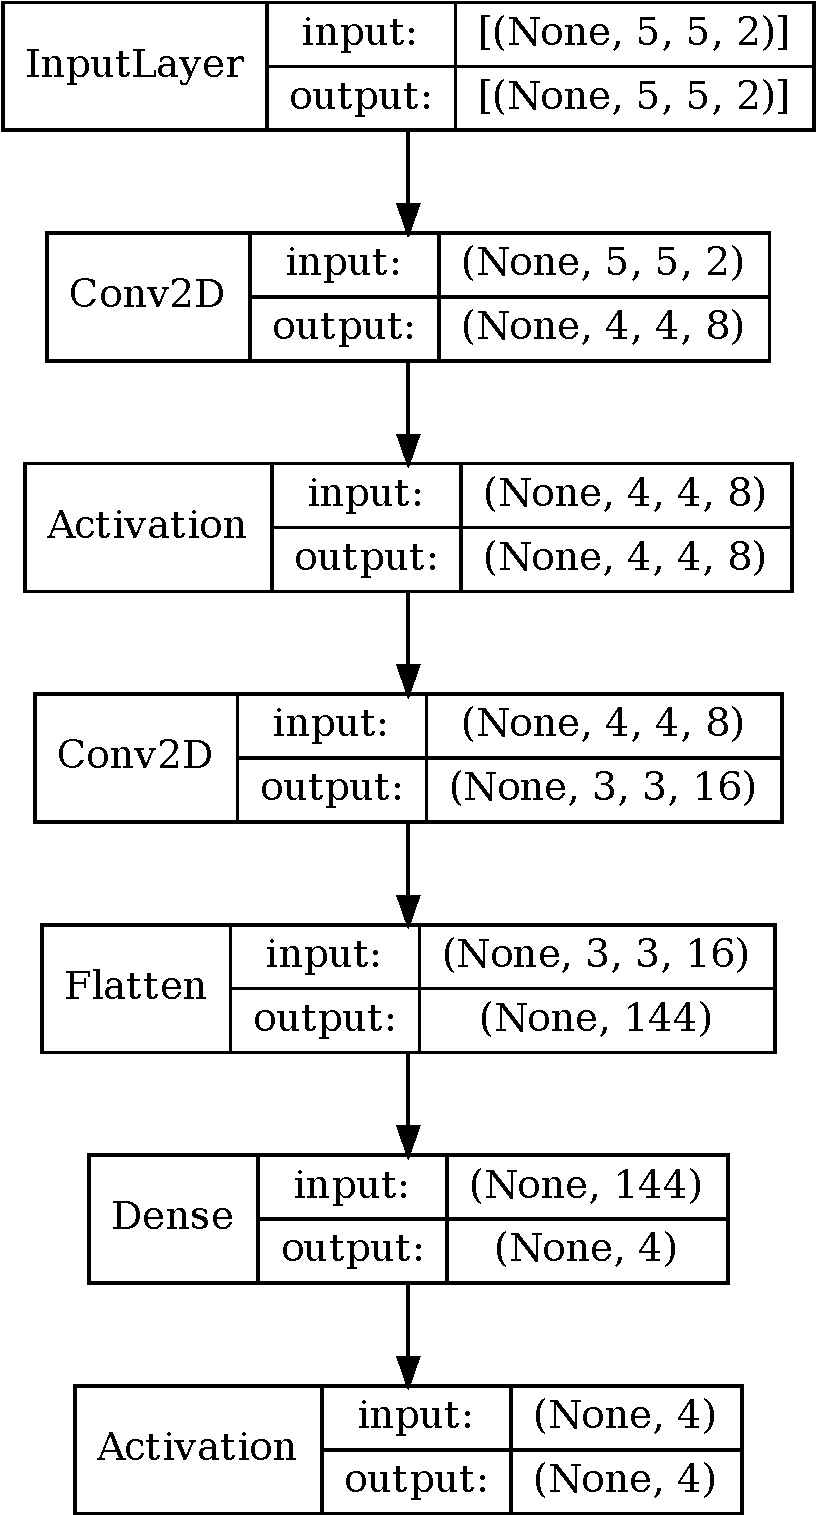
\includegraphics[width = 0.5\textwidth]{figures/dq_cnn.pdf}
		\end{figure}
		\column{0.1 \textwidth}
		\column{0.5 \textwidth}
		\begin{figure}
			\animategraphics[autoplay,loop,width=0.8\textwidth]{15}{figures/DQ/cnn_test0_}{0}{201}
		\end{figure}
	\end{columns}
\end{frame}

\begin{frame}{}{$\epsilon$-greedy Algorithm}
	The $\epsilon$-greedy algorithm is a common exploration strategy used in Deep Q learning. Balances exploration, where the agent tries out new actions and collects new data, and exploitation, where the agent uses the information it already has to select the action with the highest expected reward. The algorithm selects a random action with probability $\epsilon$ and the action with the highest Q value with probability $1-\epsilon$. The value of $\epsilon$ decreases over time to gradually shift the focus from exploration to exploitation.
\end{frame}

\begin{frame}{}{Model 2+ Incorporated $\epsilon$-exploration}

	\begin{columns}[c, onlytextwidth]
		\column{0.4 \textwidth}
		Convolutional network + $\epsilon$-greedy Algorithm during training:
		\begin{figure}
			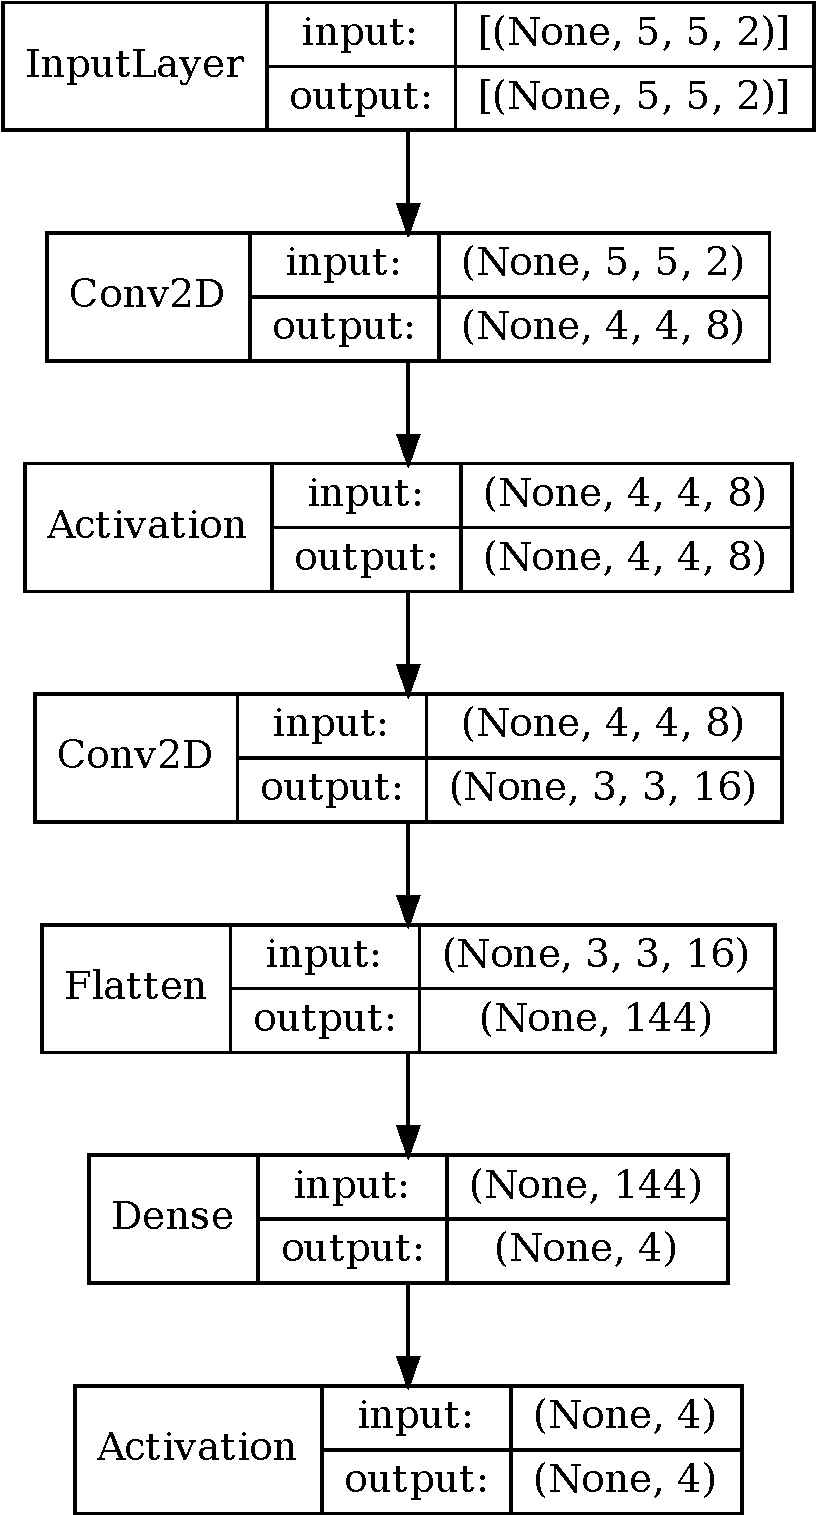
\includegraphics[width = 0.5\textwidth]{figures/dq_cnn.pdf}
		\end{figure}
		\column{0.1 \textwidth}
		\column{0.5 \textwidth}
		\begin{figure}
			\animategraphics[autoplay,loop,width=0.8\textwidth]{15}{figures/DQ/cnn_test_exp0_}{0}{201}
		\end{figure}
	\end{columns}
\end{frame}

\section{Synthetic Data Generation with Generative Adversarial Networks}
\subsection{GANS Models}
\begin{frame}
	Generative Adversarial Networks (GANs) are a type of deep learning architecture composed of two neural networks, the generator and the discriminator, that are trained in a adversarial manner. The generator network is trained to generate fake data that appears similar to real data, while the discriminator network is trained to distinguish between real and fake data. The loss for GANs is defined as a min-max game, where the generator minimizes the loss function, and the discriminator maximizes it. $D$ and $G$ represent the discriminator and generator networks, respectively, and the goal is to find the optimal configuration for $D$ and $G$ such that the generated samples appear indistinguishable from real data.

	\begin{figure}
		\centering
		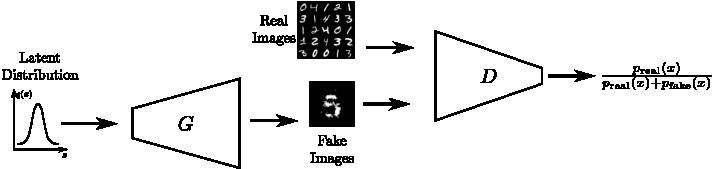
\includegraphics[width = 0.9\textwidth]{figures/GAN.pdf}
	\end{figure}
\end{frame}
\begin{frame}
	The loss of a  (GAN) is defined as a minimax game between the generator and discriminator models. The generator aims to generate samples that are indistinguishable from real samples, while the discriminator aims to distinguish the generated samples from real samples. The loss function for the generator is defined as $-\log(D(G(z)))$, where $D$ is the discriminator model and $G(z)$ is the generator's output for a random noise vector $z$. The loss function for the discriminator is defined as $\log(D(x)) + \log(1 - D(G(z)))$, where $x$ is a real sample.
	$$
		\min_D \max_G \mathbb{E}_{x\sim p_{\mathrm{real}}}\left[\log(D(x))\right]  +  \mathbb{E}_{z\sim q}\left[ \log(1 - D(G(z)))\right]
	$$

	\begin{figure}
		\centering
		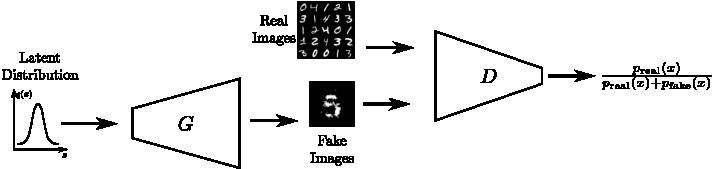
\includegraphics[width = 0.9\textwidth]{figures/GAN.pdf}
	\end{figure}
\end{frame}

\subsection{MNIST Generation}
\begin{frame}
	\begin{columns}[c, onlytextwidth]
		\column{0.5\textwidth}
		\centering $G$
		\begin{figure}
			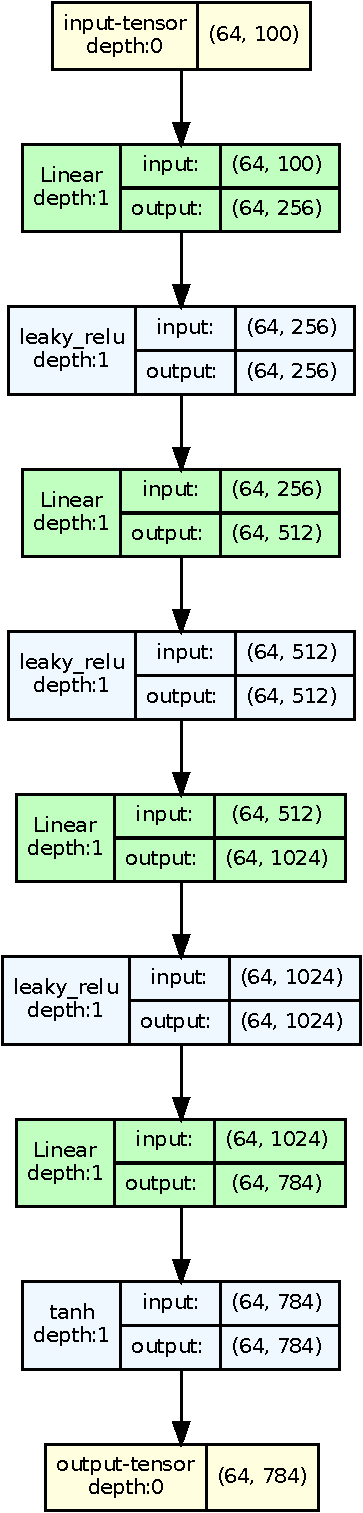
\includegraphics[width=0.2\textwidth]{figures/F.pdf}
		\end{figure}

		\column{0.5\textwidth}
		\centering $D$
		\begin{figure}
			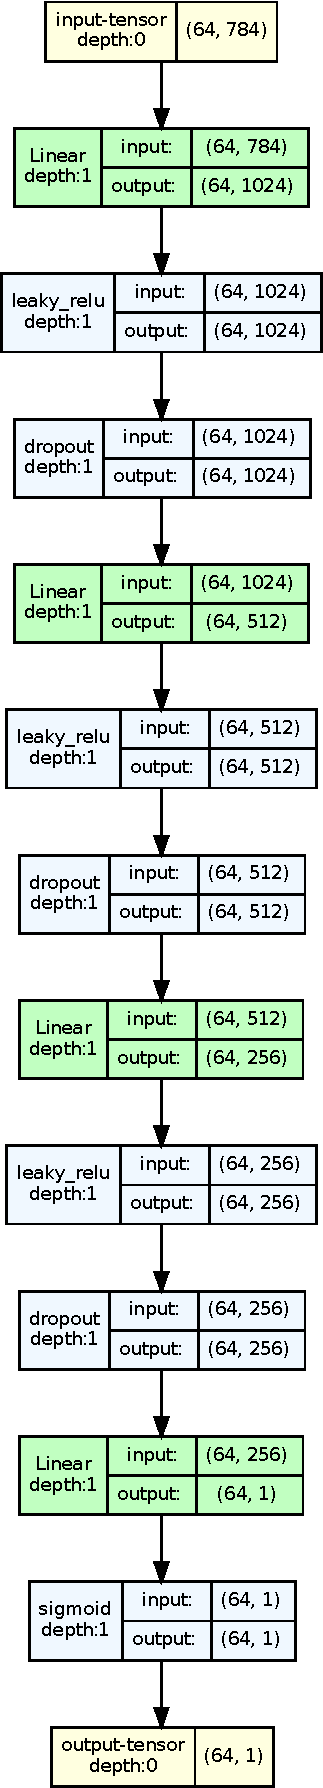
\includegraphics[width=0.2\textwidth]{figures/D.pdf}
		\end{figure}
	\end{columns}
\end{frame}

\begin{frame}
	\begin{figure}
		\centering
		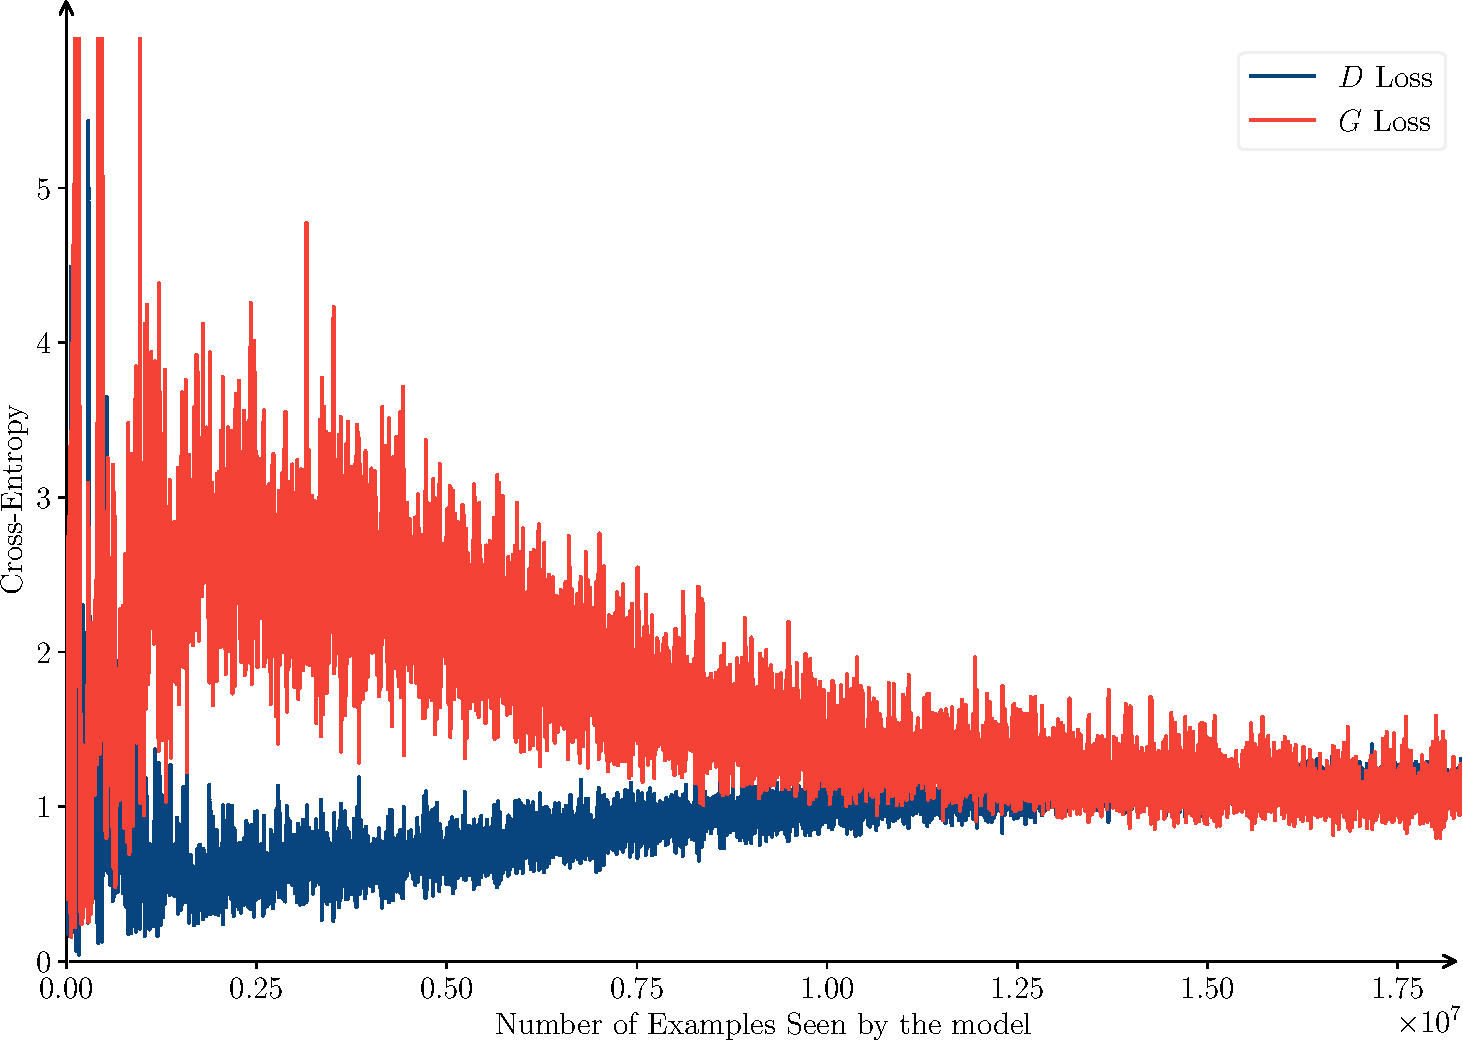
\includegraphics[width = 0.6 \textwidth]{figures/gan_loss.pdf}
	\end{figure}
\end{frame}

\begin{frame}
	\begin{figure}
		\animategraphics[autoplay,loop,width=0.4\textwidth]{15}{figures/GAN/sample_}{1}{305}
	\end{figure}
\end{frame}
\section{Sentiment Analysis with Transformers and GRU}
\subsection{Bert}
\begin{frame}
	BERT (Bidirectional Encoder Representations from Transformers) is a pre-trained language model developed by Google in 2018. It is a transformer-based architecture that uses a masked language modeling task to generate a deep understanding of the contextual relationships between words in a sentence. BERT can be fine-tuned for various NLP tasks such as sentiment classification by adding a classification layer on top of its pre-trained representations. The model has achieved state-of-the-art performance in a wide range of NLP tasks, making it a popular choice for sentiment analysis.\newline

	A bidirectional transformer is a type of transformer architecture in natural language processing (NLP) where information from both past and future contexts is taken into consideration when making predictions. This is achieved by processing the input sequence in two directions, starting from the beginning and the end of the sequence, and concatenating the outputs to obtain the final representation. This allows the model to capture the context both in the forward and backward directions, providing a more comprehensive representation of the input sequence.
\end{frame}


\begin{frame}
	BERT model consists of multiple transformer encoder blocks, with a self-attention mechanism, a feedforward neural network and layer normalization, stacked on top of each other. It also includes a positional encoding component to capture the relative position of tokens in a sequence, and a segment encoding component to differentiate between different sequences within the same input.
	\begin{figure}
		\centering
		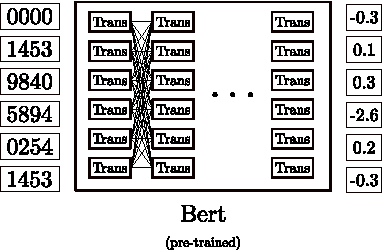
\includegraphics[width = 0.6 \textwidth]{figures/bert.pdf}
	\end{figure}
\end{frame}
\begin{frame}{}{Training Bert}

	Bert is trained on two tasks, the masked language model and the next sentence prediction. In the masked language model task, a portion of the input sequence is masked and the model must predict the original token based on its context. In the next sentence prediction task, the model receives a pair of sentences and must predict whether the second sentence follows the first one in the context of the input text. Both of these tasks are used to train Bert to understand the context of words in a sentence and how they relate to each other, allowing it to perform well on a wide range of natural language processing tasks.
	\begin{figure}
		\centering
		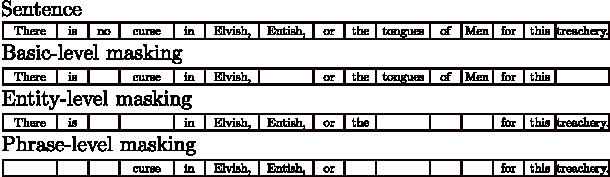
\includegraphics[width = 0.8 \textwidth]{figures/masking.pdf}
	\end{figure}
\end{frame}
\subsection{Sentiment Analysis}
\begin{frame}
	Bert can be fine-tuned for sentiment analysis by adding a classifier layer on top of the pretrained Bert model. The layer is trained on a labeled sentiment analysis dataset to predict the sentiment of a given input sequence, which can be a sentence, paragraph, or document. Fine-tuning the model allows it to learn the specific nuances of sentiment in the target task and produce improved results compared to using the pre-trained model alone.
	\begin{figure}
		\centering
		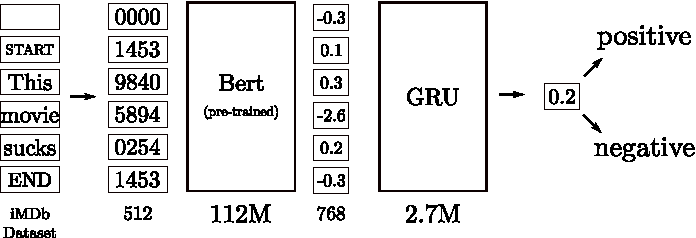
\includegraphics[width = 0.6 \textwidth]{figures/Bertsentiment.pdf}
	\end{figure}
\end{frame}
\begin{frame}
	\begin{figure}
		\centering
		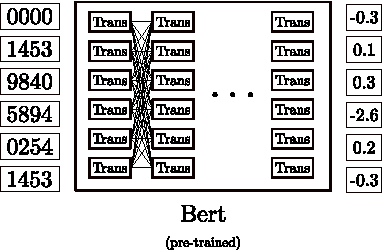
\includegraphics[width = 0.6 \textwidth]{figures/bert.pdf}
	\end{figure}
\end{frame}
\begin{frame}
	\begin{figure}
		\centering
		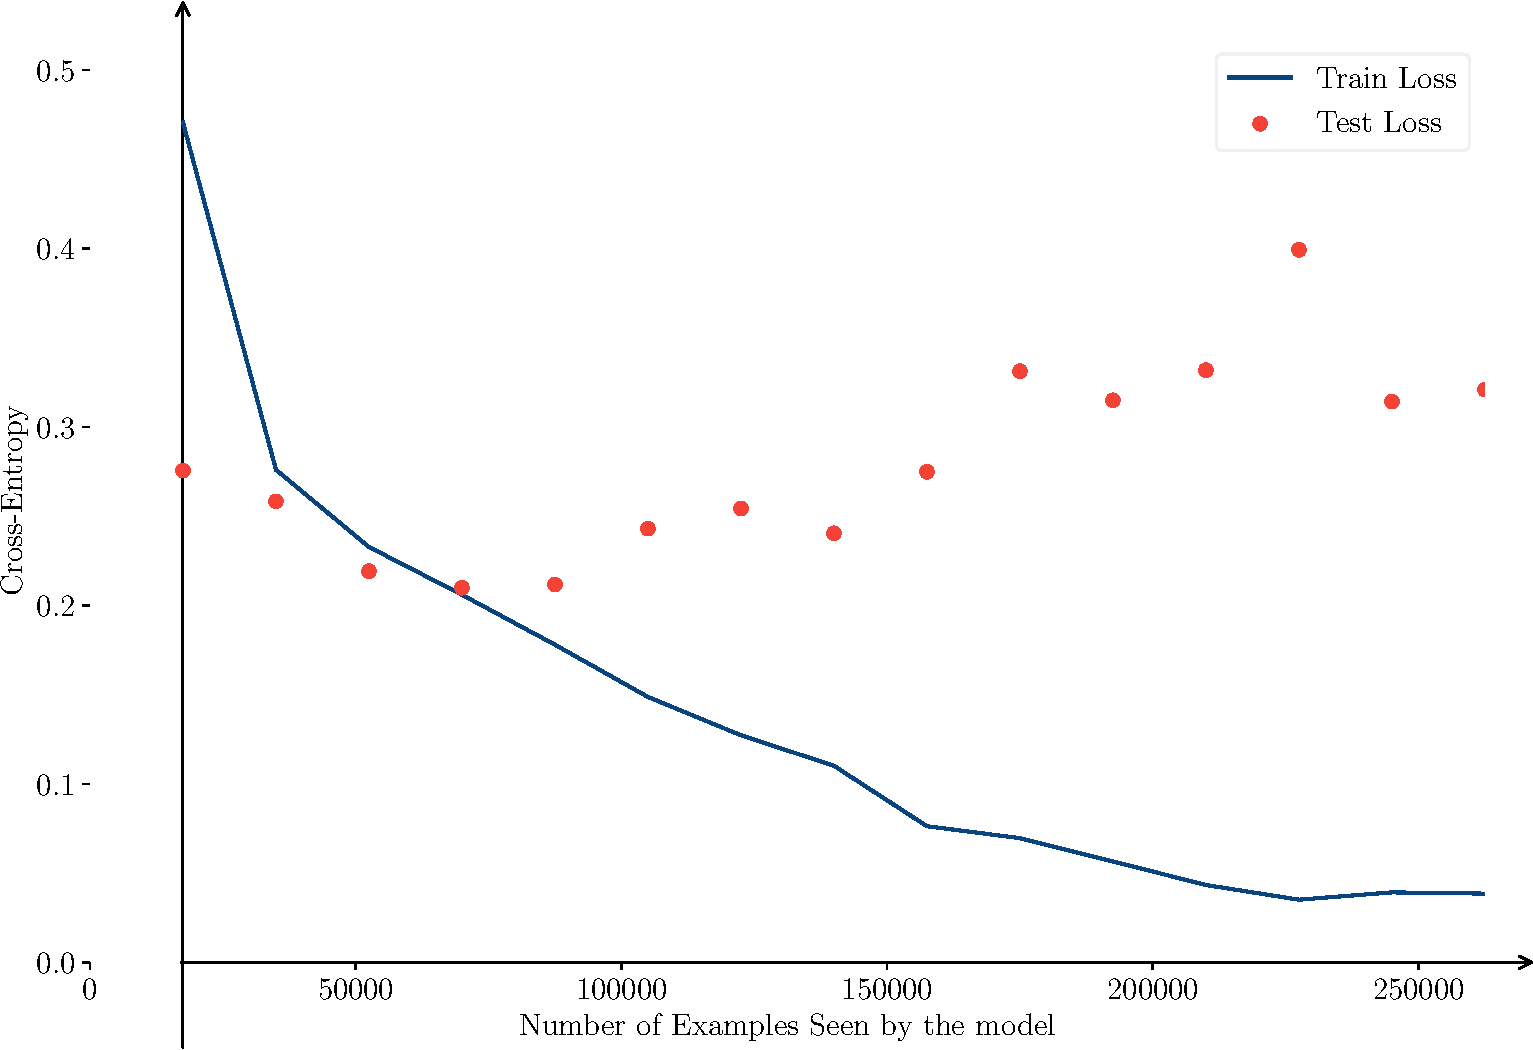
\includegraphics[width = 0.6 \textwidth]{figures/bert_res.pdf}
	\end{figure}
\end{frame}

\begin{frame}
	\begin{figure}
		\centering
		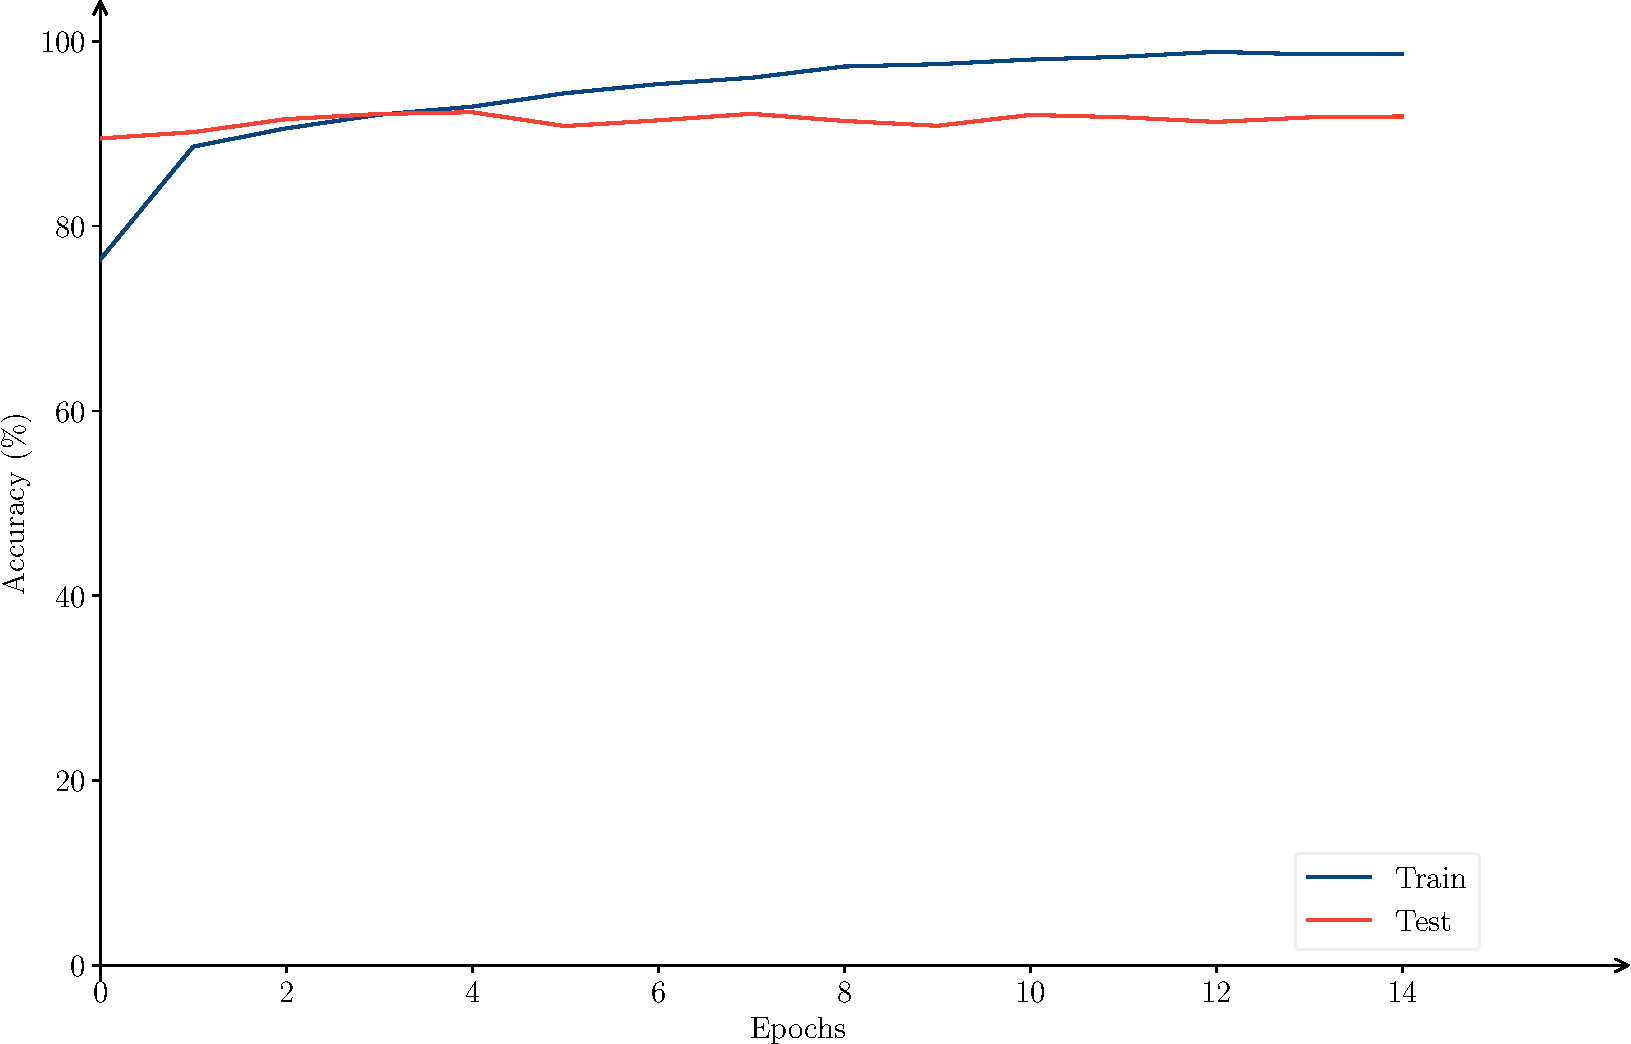
\includegraphics[width = 0.6 \textwidth]{figures/bert_acc.pdf}
	\end{figure}
\end{frame}

\begin{frame}
	\begin{figure}
		\centering
		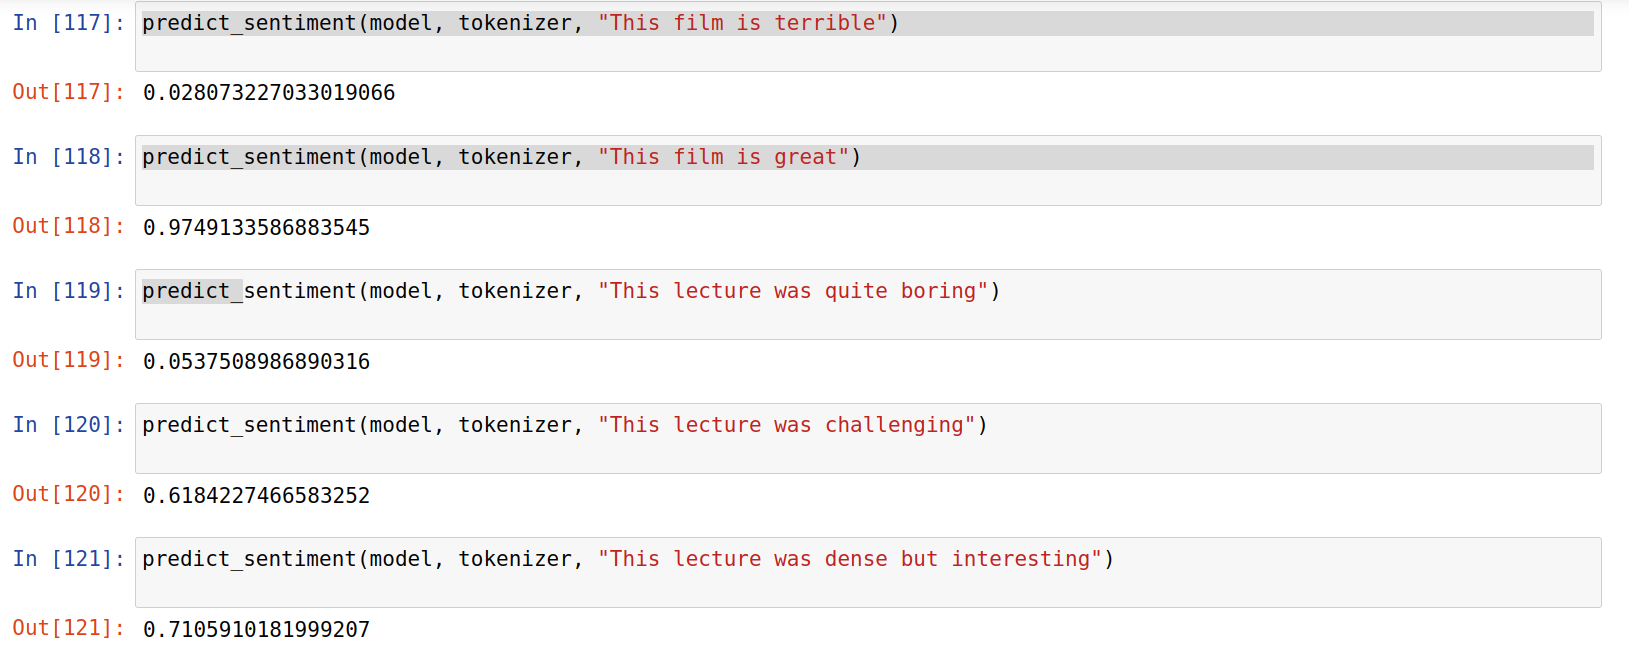
\includegraphics[width = 0.7 \textwidth]{figures/bert_sen.png}
	\end{figure}
\end{frame}





\section{Density Estimation with Normalizing Flows}
\subsection{Estimating Density}
\begin{frame}
	In Machine Learning, the task of \emph{density estimation} consists in estimating the probability density function of a random variable from a set of observations. This is a fundamental problem in statistics and machine learning, with applications in a wide range of fields, including anomaly detection, clustering, and generative modeling. There are several methods for density estimation, including parametric models, non-parametric models, and deep learning models. In this section, we will focus on a specific type of deep learning model called Normalizing Flows, which is used for density estimation and generative modeling.
	\vskip 5pt
	\begin{figure}
		\centering
		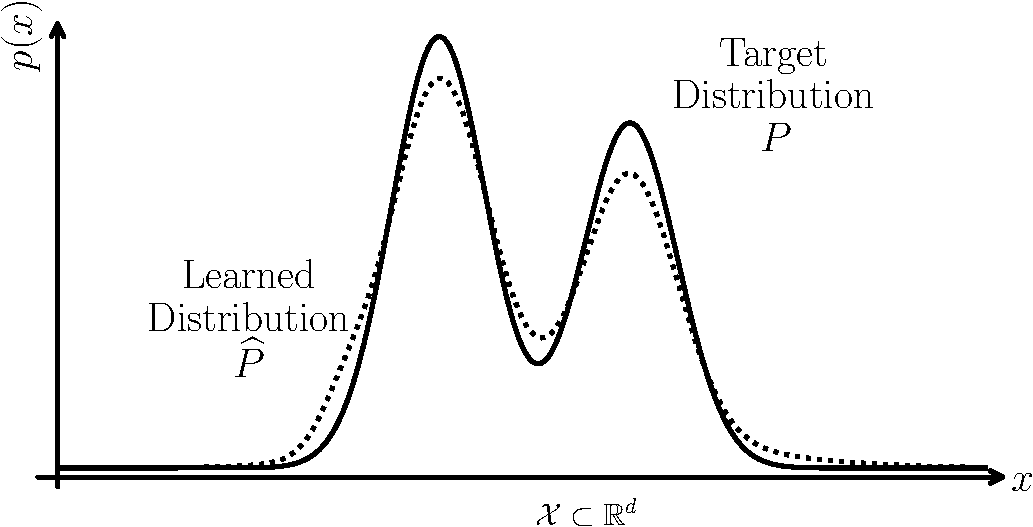
\includegraphics[width = 0.5\textwidth]{figures/targetnproposal.pdf}
	\end{figure}

\end{frame}

\subsection{Normalizing Flows}




\begin{frame}{}{Overview}
	A Normalizing Flow is usually seen as:
	\begin{itemize}
		\item a  {\em generative model},
		\item a {\em bijective mapping},
		\item an {\em invertible neural network},
		\item a {\em density estimator}.
	\end{itemize}
\end{frame}
\begin{frame}{}{Overview}
	\begin{figure}
		\centering
		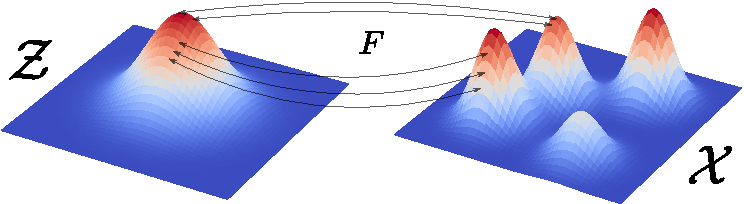
\includegraphics[width = \textwidth]{figures/Distribution_NF.pdf}
		\caption{A mapping between two probability distributions\\Point to point}
	\end{figure}
\end{frame}
\begin{frame}{}{Overview}
	\begin{figure}
		\centering
		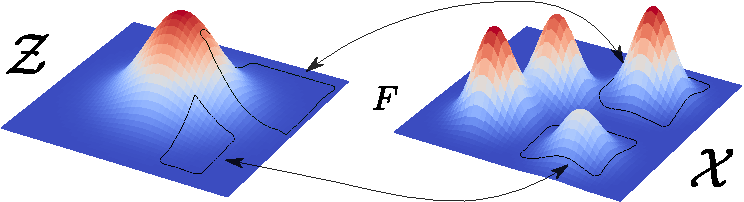
\includegraphics[width = \textwidth]{figures/Distribution_NF2.pdf}
		\caption{A mapping between two probability distributions\\Subset to subset}
	\end{figure}
\end{frame}

\begin{frame}{}{Mathematical Framework}
	\begin{block}{Normalizing Flow}
		A Normalizing Flow is a bijective function between a data space $\mathcal{X}$ and a latent space $\mathcal{Z}$, both subset of $\mathbb{R}^d$.
		$$
			\begin{array}{rccl}
				F : & \mathcal{X} & \longmapsto & \mathcal{Z} \\
				    & x           & \longmapsto & z = F(x)
			\end{array}
		$$
	\end{block}
	\begin{block}{Data and Latent Distributions}
		In theory, a NF maps a target distribution $P$, ie the data distribution to a  simple latent distribution $Q$.
	\end{block}
	Usually, $Q$ is set to be a Normal Gaussian multivariate distribution $\mathcal{N}(0_d,I_d)$. $p$ and $q$ are respectivelly the probability densities of $P$ and $Q$.
\end{frame}

\begin{frame}{}{How does it work ?}
	In practice, the mapping is {\em  not perfect}. $P^*$ induces a distribution $Q$ and similarly, the latent distribution $Q$ induces $\widehat P$,  which is the learned distribution. The forward pass $F$ is called the {\em Normalizing } direction while the inverse pass $F^{-1}$ is called the {\em Generative} direction.
	\vskip 5pt
	\begin{figure}
		\centering
		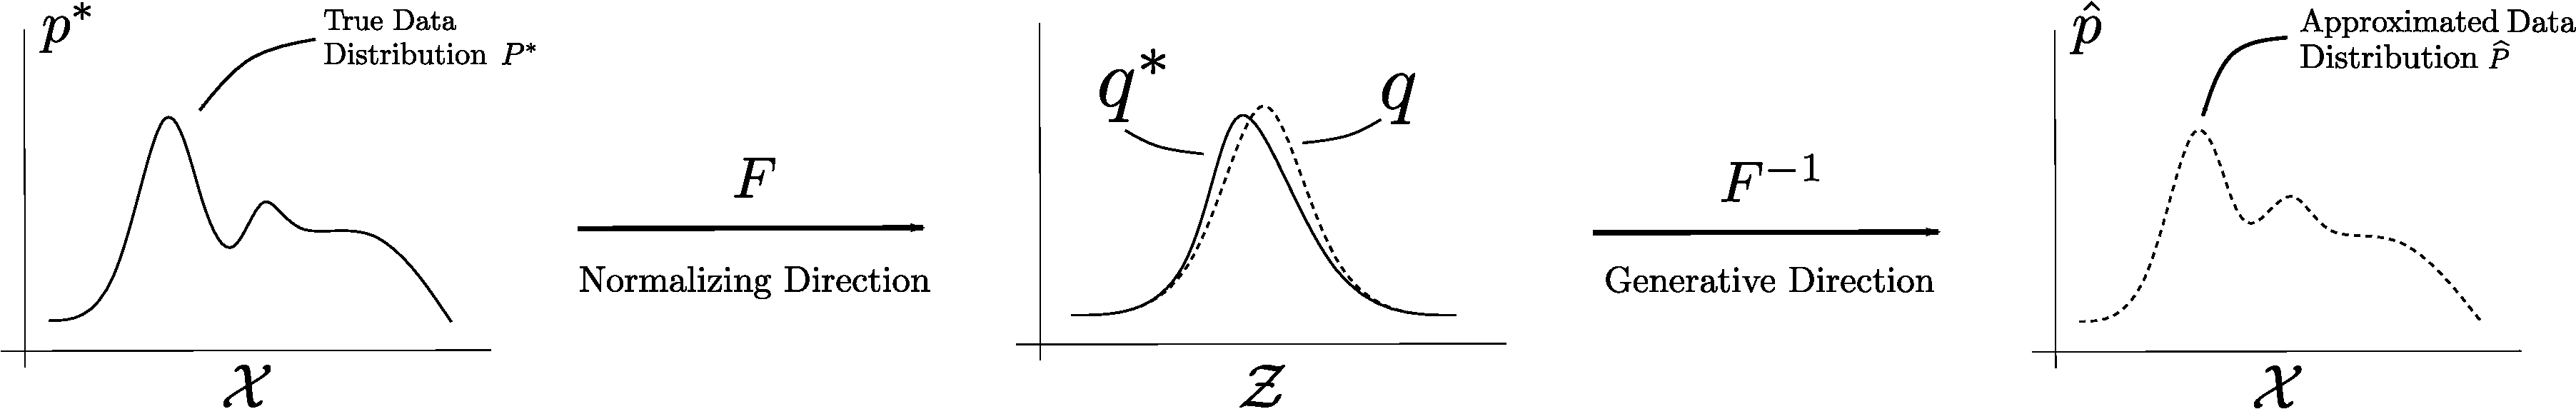
\includegraphics[width = \textwidth]{figures/nf.pdf}
		\caption{1D Normalizing Flow process.}
	\end{figure}
\end{frame}

\begin{frame}{}{Induced Probabilities ? }
	\begin{block}{Change of Variable Formula}
		For a bijective and continuous fonction $F$ and a latent distribution $Q$, the distribution induced by $Q$ and $F$ is defined through the {\em change of variable formula}:
		\begin{equation}
			\label{eq:cov}
			\forall x \in \mathcal{X}, \quad \hat p(x) = \vert \det \mathrm{Jac}_F(x)\vert ~ q(F(x)).
		\end{equation}
	\end{block}
\end{frame}

\begin{frame}{}{Induced Probabilities ? }
	$$\forall x \in \mathcal{X}, \quad \hat p(x) = \vert \det \mathrm{Jac}_F(x)\vert ~ q(F(x)).$$
	\only<1>{
		\begin{figure}
			\centering
			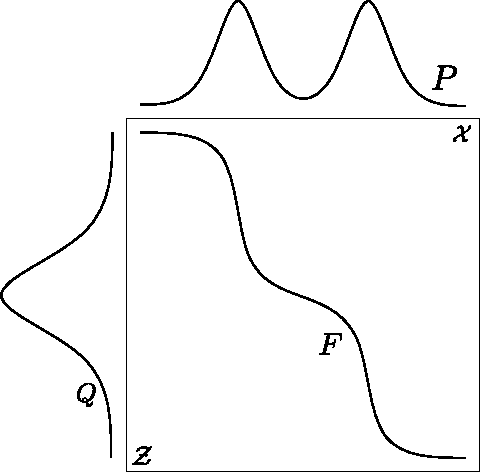
\includegraphics[width = 0.4\textwidth]{figures/monge.pdf}
		\end{figure}
	}
	\only<2>{
		\begin{figure}
			\centering
			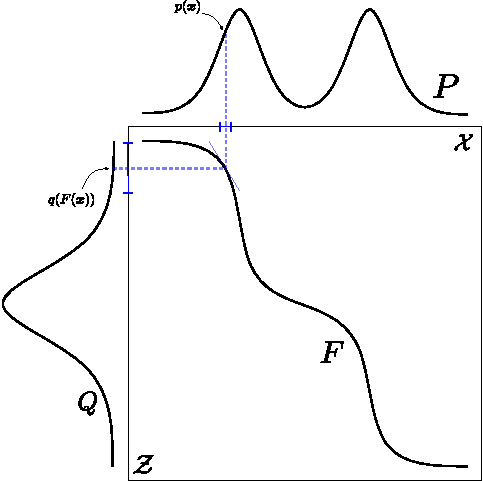
\includegraphics[width = 0.4\textwidth]{figures/monge_L1.pdf}
		\end{figure}
	}
	\only<3>{
		\begin{figure}
			\centering
			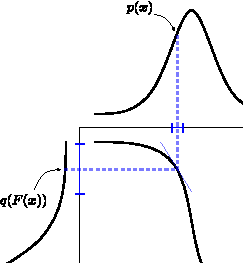
\includegraphics[width = 0.4\textwidth]{figures/monge_L1_cropped.pdf}
		\end{figure}
	}
	\only<4>{
		\begin{figure}
			\centering
			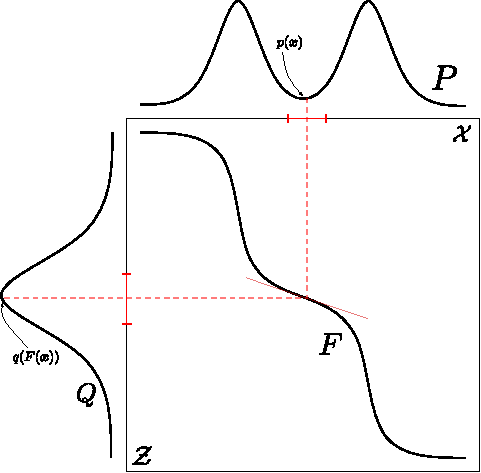
\includegraphics[width = 0.5\textwidth]{figures/monge_L2.pdf}
		\end{figure}
	}
	\only<5>{
		\begin{figure}
			\centering
			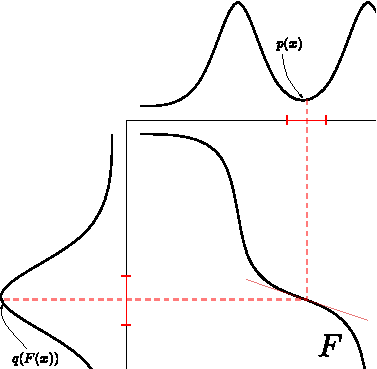
\includegraphics[width = 0.4\textwidth]{figures/monge_L2_cropped.pdf}
		\end{figure}
	}

\end{frame}

\begin{frame}{}{Density Estimation}
	To perfom density estimation:
	\begin{enumerate}
		\item Draw $x \sim P^*$,
		\item Compute $F(x)$ and $\vert \det \mathrm{Jac}_F(x)\vert$,
		\item Compute $\widehat{p}(x) = q(F(x))\vert \det \mathrm{Jac}_F(x)\vert $.
	\end{enumerate}
	\begin{figure}
		\centering
		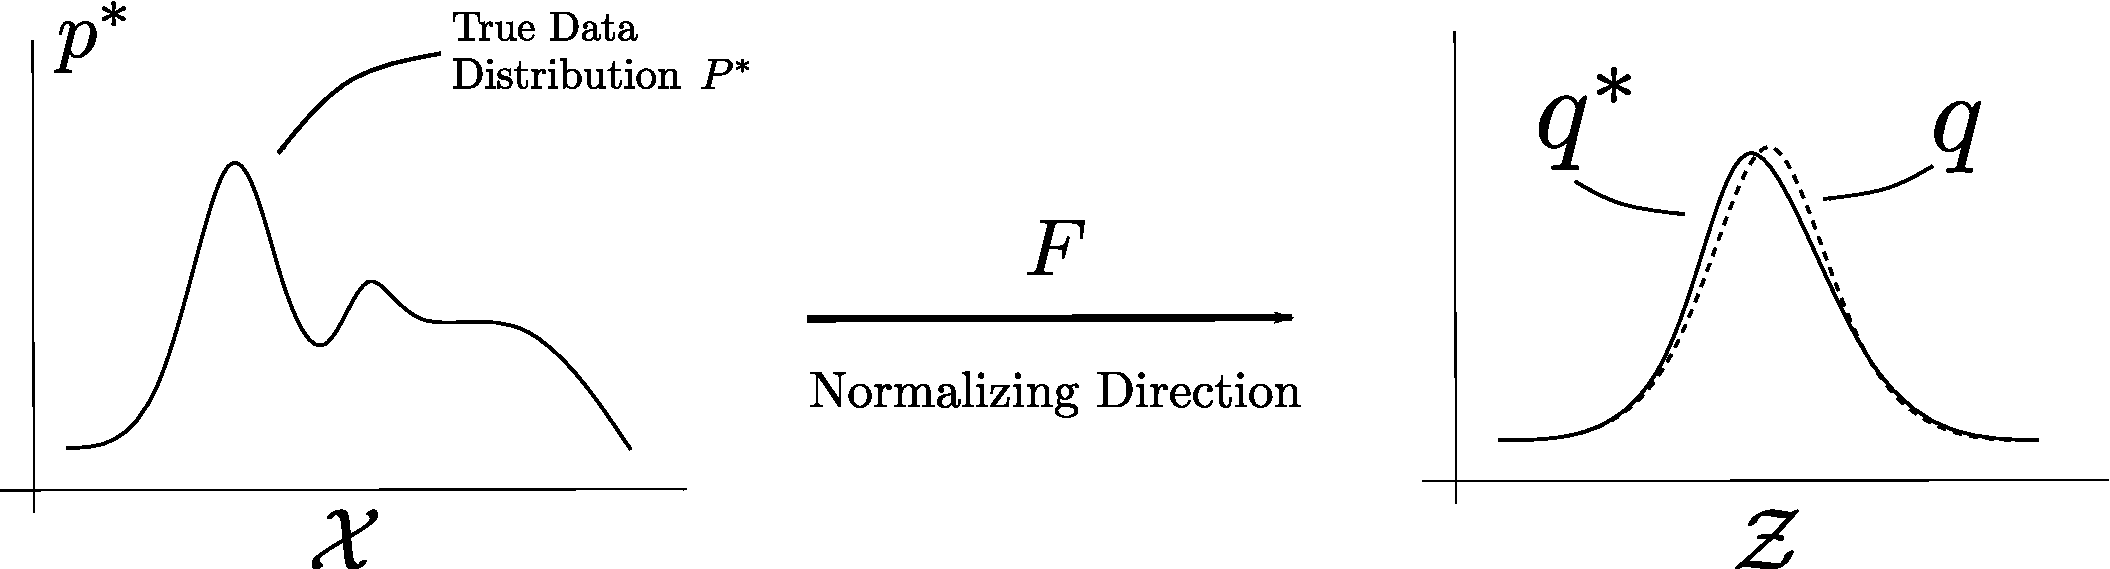
\includegraphics[width = 0.9\textwidth]{figures/nf_de.pdf}
		\caption{1D Normalizing Process of Density Estimation.}
	\end{figure}
\end{frame}

\begin{frame}{}{Data Generation}
	To perform data generation:
	\begin{enumerate}
		\item Draw $z \sim Q$,
		\item Compute $x = F^{-1}(x)$.
	\end{enumerate}
	\begin{figure}
		\centering
		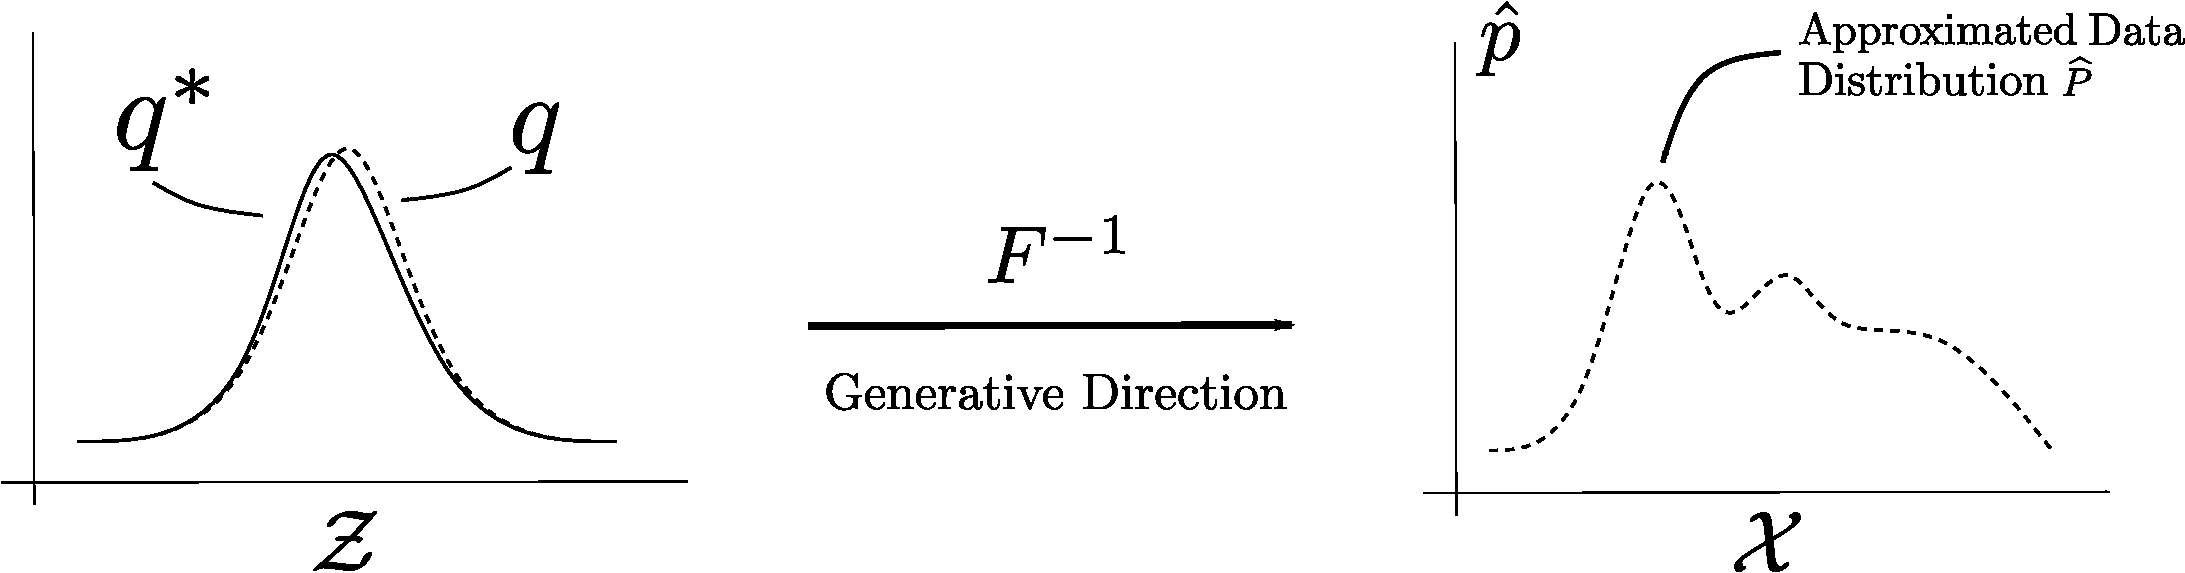
\includegraphics[width = 0.9\textwidth]{figures/nf_gen.pdf}
		\caption{1D Normalizing Flow process of Generation.}
	\end{figure}
\end{frame}



\begin{frame}{}{Log-Likelihood}
	\begin{exampleblock}{Loss}
		The objective is to approximate $P^*$ with $\widehat P$. We can minimize the Kullback-Leiber Divergence :
		\begin{equation*}
			\theta = \argmin_\theta \mathcal{D}_{\mathrm{KL}}(P^*\Vert \widehat{P}).
		\end{equation*}
		This is equivalent to maximizing the log likelihood :
		\begin{equation*}
			\theta = \argmax_\theta \mathbb{E}_{x\sim \mathcal{X}} \left[\log\widehat{p}(x)\right].
		\end{equation*}
	\end{exampleblock}
\end{frame}

\begin{frame}{}{Log-Likelihood}
	$$ \mathcal{D}_{\mathrm{KL}}(P^*\Vert \widehat{P}) = \int_{\mathcal{X}}p^*(x)\log\left(\frac{p^*(x)}{\widehat p(x)}\right)dx$$
	\vfill
	\vskip 75pt
	$$ \mathrm{nll} =- \mathbb{E}_{x\sim\mathcal{X}}\left[\log \widehat p (x)\right]$$
\end{frame}

\begin{frame}{}{Learning steps}
	\begin{figure}
		\centering
		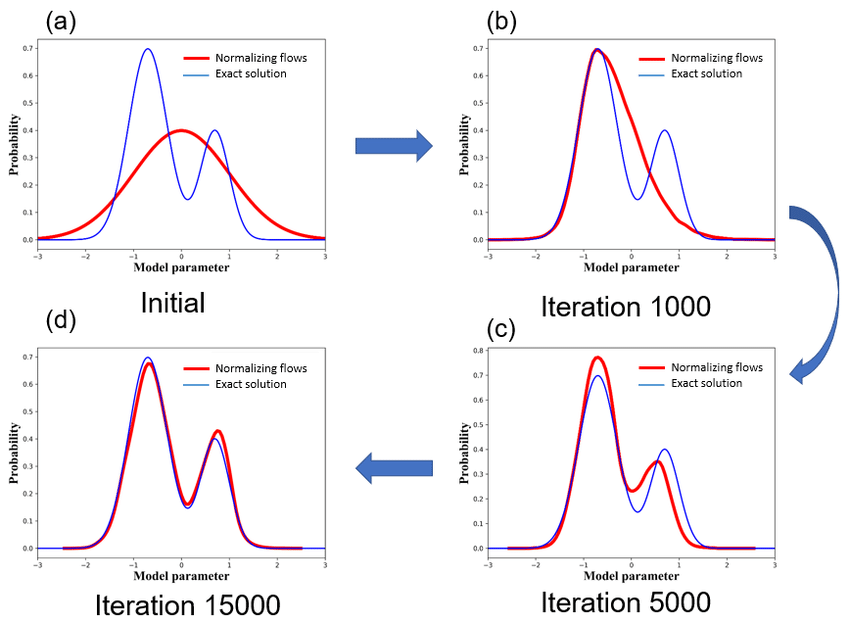
\includegraphics[width = 0.65\textwidth]{figures/learning.png}
		\caption{Learning Process for a 1D Normalizing Flow.}
	\end{figure}
\end{frame}


\section{Image Segmentation with U-Net}
\subsection{Image Segmentation}

\begin{frame}
	Image segmentation is the process of partitioning an image into multiple segments or regions based on the characteristics of the pixels. It is a fundamental task in computer vision and has applications in various fields, including medical imaging, autonomous driving, and satellite image analysis. There are several methods for image segmentation, including thresholding, clustering, and deep learning-based approaches. In this section, we will focus on a deep learning model called U-Net, which is commonly used for image segmentation tasks.

	\begin{figure}
		\centering
		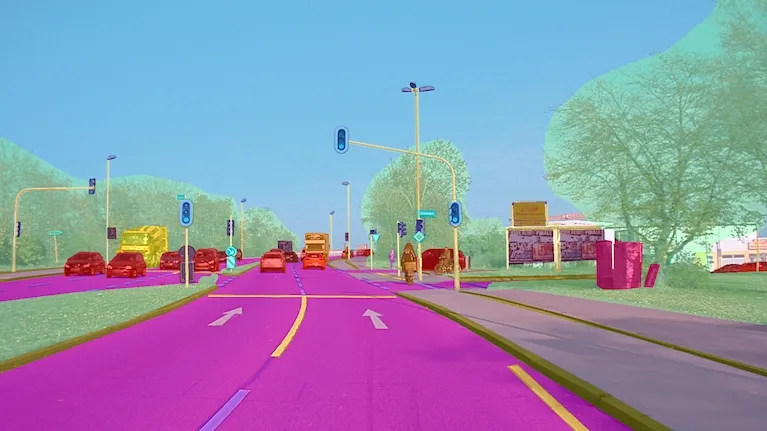
\includegraphics[width = 0.6\textwidth]{figures/imageseg.png}
	\end{figure}
\end{frame}

\begin{frame}{}{Applications of Image Segmentation}
	Image segmentation has a wide range of applications in computer vision and image processing, including:
	\begin{itemize}
		\item Medical Imaging: Segmentation of organs, tumors, and other structures in medical images.
		\item Autonomous Driving: Segmentation of objects such as cars, pedestrians, and road signs in images captured by autonomous vehicles.
		\item Satellite Image Analysis: Segmentation of land cover types, buildings, and other features in satellite images.
		\item Object Detection: Segmentation of objects in images to localize and classify them.
		\item Image Editing: Segmentation of objects for image editing tasks such as background removal and image compositing.
	\end{itemize}
\end{frame}

\begin{frame}{}{Type of Segmentations}
	\begin{minipage}[t]{0.48\textwidth}

		Image segmentation can be broadly classified into two types: semantic segmentation and instance segmentation.
		\begin{itemize}
			\item \textbf{Semantic Segmentation:} Semantic segmentation assigns a class label to each pixel in an image, such as road, car, person, etc. The goal is to partition the image into semantically meaningful regions.
			\item \textbf{Instance Segmentation:} Instance segmentation goes a step further than semantic segmentation by distinguishing between different instances of the same class. It assigns a unique label to each object instance in the image.
		\end{itemize}
	\end{minipage}
	\hfill
	\begin{minipage}[t]{0.48\textwidth}
		\begin{figure}
			\centering
			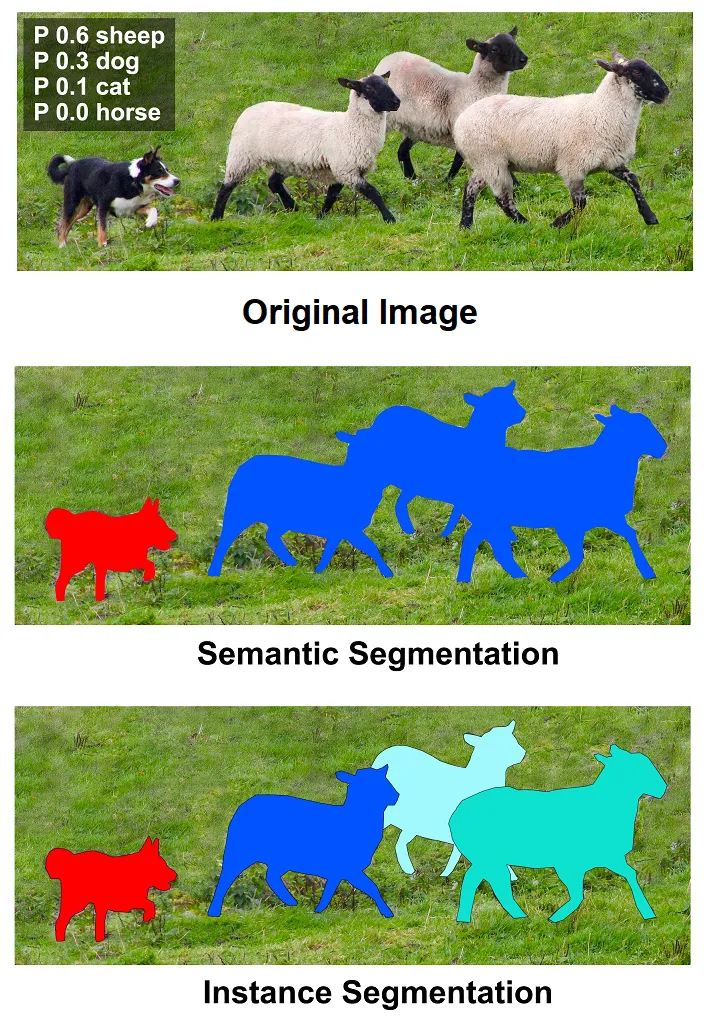
\includegraphics[width = 0.6\textwidth]{figures/typeseg.png}
		\end{figure}
	\end{minipage}
\end{frame}

\subsection{U-Net Architecture}
\begin{frame}
	U-Net is a convolutional neural network architecture designed for image segmentation tasks. It consists of an encoder-decoder structure with skip connections that allow the model to capture both local and global features in the input image.
	\begin{figure}
		\centering
		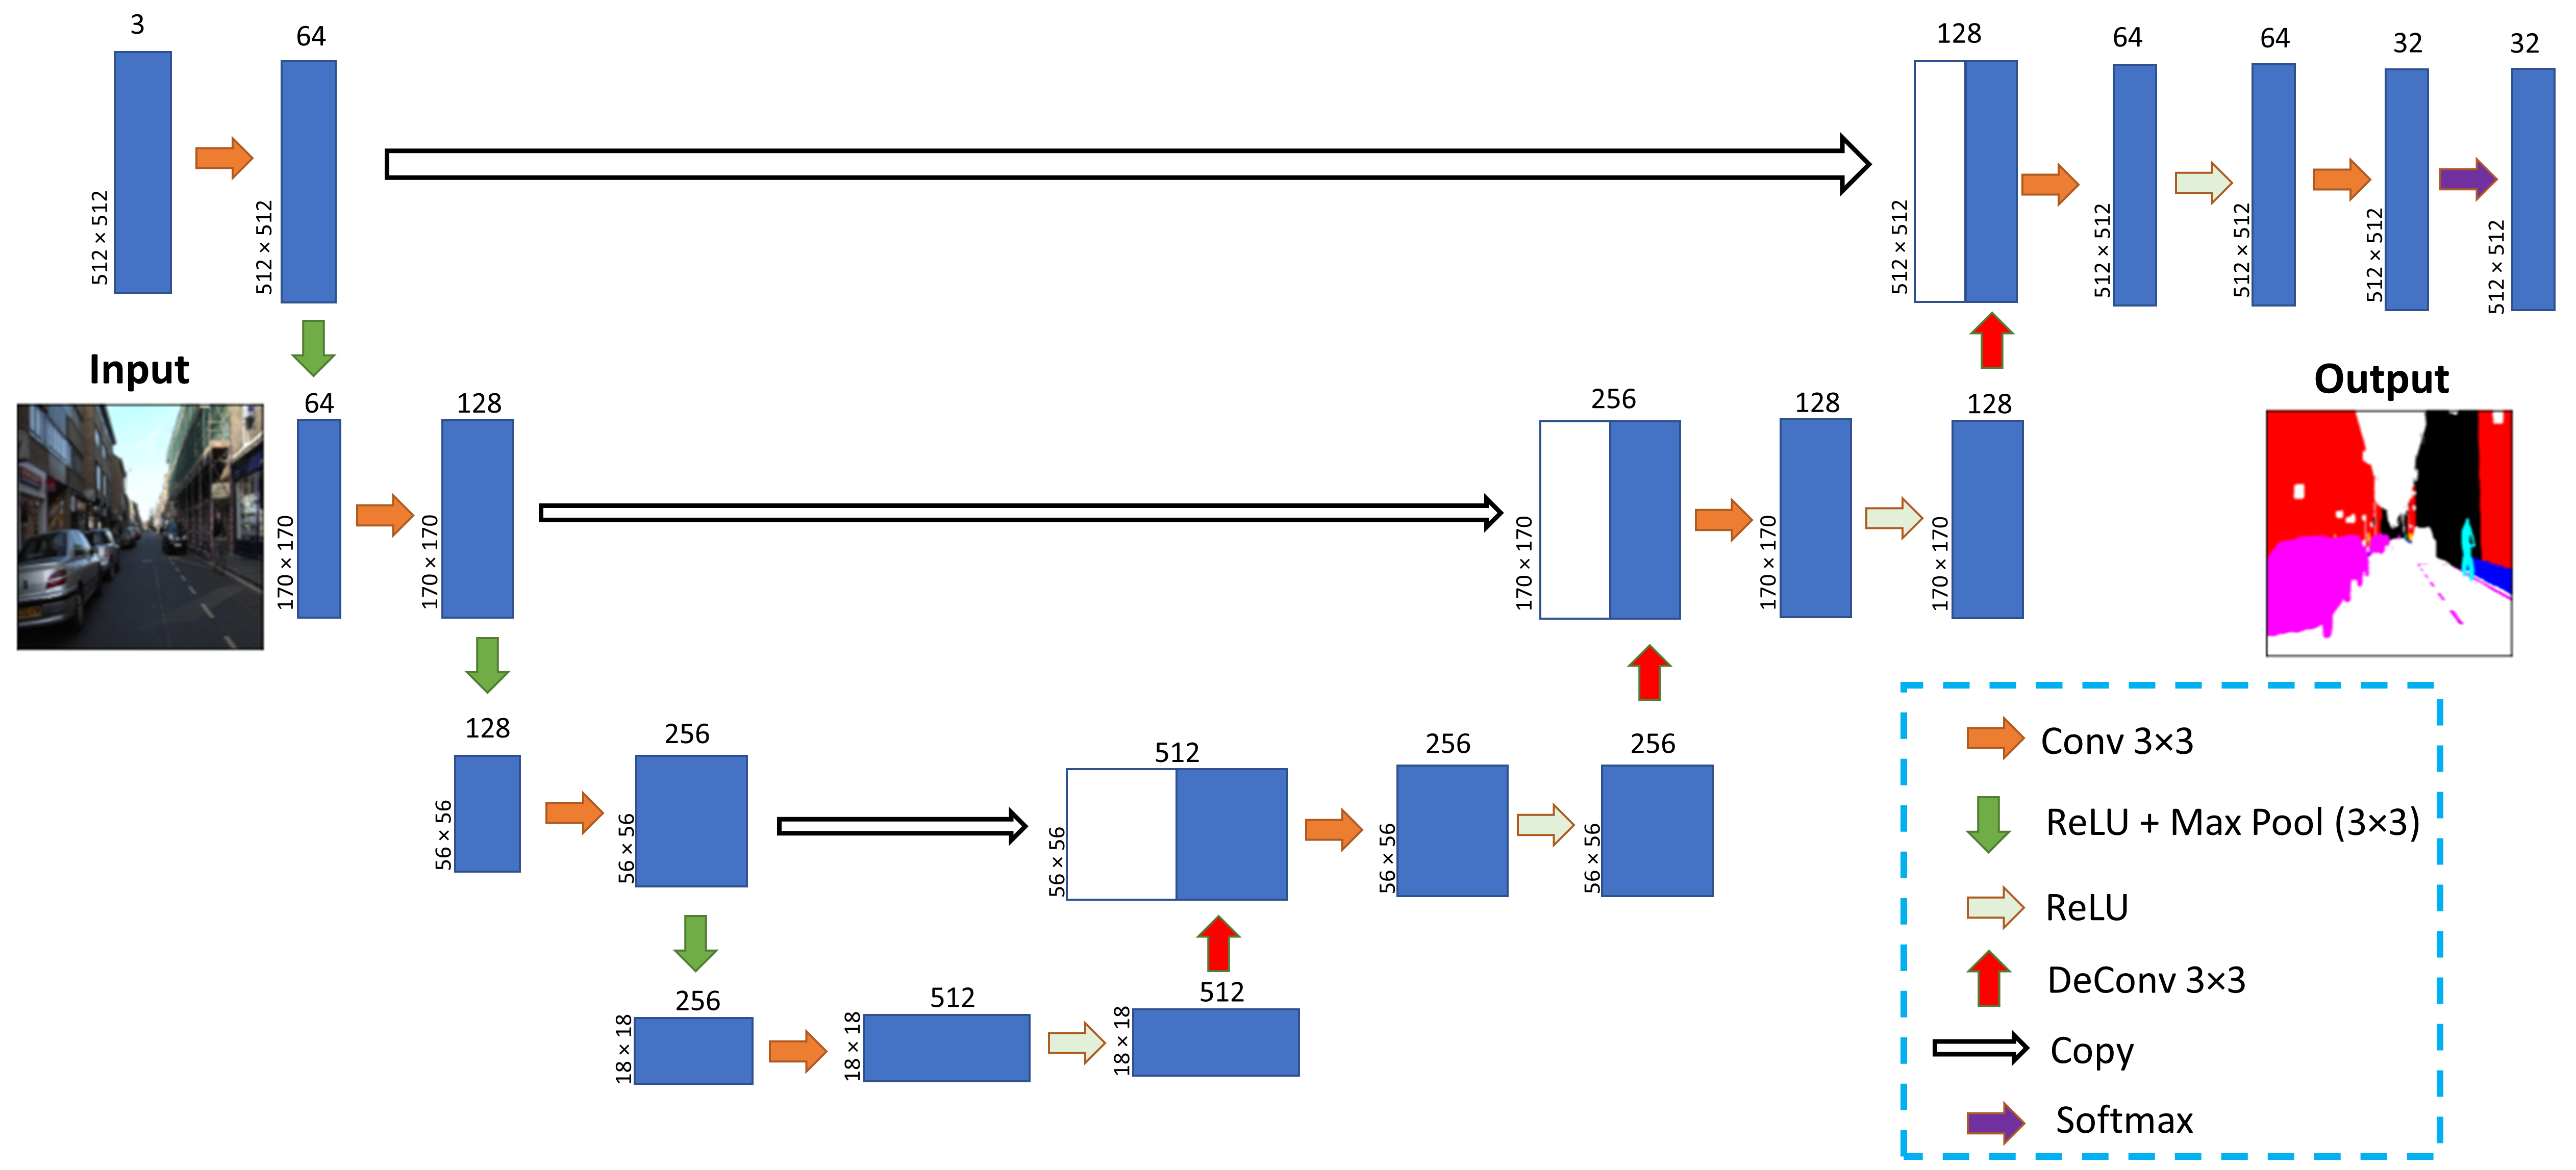
\includegraphics[width = 0.6\textwidth]{figures/U_Net_arch.png}
	\end{figure}
\end{frame}

\begin{frame}{}{Loss Functions}
	3 main loss functions are used for image segmentation tasks:
	\begin{itemize}
		\item \textbf{Categorical Cross-Entropy Loss:} Used for multi-class segmentation tasks where each pixel is classified into one of multiple classes.
		      \only<2>{
		      $$\mathcal{L} = -\frac{1}{N}\sum_{i=1}^{N}\sum_{c=1}^{C}y_{i,c}\log(\hat{y}_{i,c})$$
		      }
		\item \textbf{Dice Loss:} A similarity-based loss function that measures the overlap between the predicted segmentation mask and the ground truth mask.
		      \only<3>{
			      $$\mathcal{L} = 1 - \frac{2\sum_{i=1}^{N}y_i\hat{y}_i}{\sum_{i=1}^{N}y_i + \sum_{i=1}^{N}\hat{y}_i}$$
		      }
		\item \textbf{Shaped aware Loss:} A loss function that penalizes the model for making errors near the object boundaries, where the segmentation is most critical.
		      \only<4>{
		      $$\mathcal{L} = -w(x)\left[\frac{1}{N}\sum_{i=1}^{N}\sum_{c=1}^{C}y_{i,c}\log(\hat{y}_{i,c})\right]$$
		      with $w(x)$ a weight function that assigns higher weights to pixels near the object boundaries.
		      }
	\end{itemize}
\end{frame}

